%%%%%%%%%%%%%%%%%%%%%%%%%%%%%%%%%%%%%%%%%%%%%%%%%%%%%%%%%%%%%%%%%%%%%%%%%%%%%
%%%
%%% File: utthesis2.doc, version 2.0jab, February 2002
%%%
%%% Based on: utthesis.doc, version 2.0, January 1995
%%% =============================================
%%% Copyright (c) 1995 by Dinesh Das.  All rights reserved.
%%% This file is free and can be modified or distributed as long as
%%% you meet the following conditions:
%%%
%%% (1) This copyright notice is kept intact on all modified copies.
%%% (2) If you modify this file, you MUST NOT use the original file name.
%%%
%%% This file contains a template that can be used with the package
%%% utthesis.sty and LaTeX2e to produce a thesis that meets the requirements
%%% of the Graduate School of The University of Texas at Austin.
%%%
%%% All of the commands defined by utthesis.sty have default values (see
%%% the file utthesis.sty for these values).  Thus, theoretically, you
%%% don't need to define values for any of them; you can run this file
%%% through LaTeX2e and produce an acceptable thesis, without any text.
%%% However, you probably want to set at least some of the macros (like
%%% \thesisauthor).  In that case, replace "..." with appropriate values,
%%% and uncomment the line (by removing the leading %'s).
%%%
%%%%%%%%%%%%%%%%%%%%%%%%%%%%%%%%%%%%%%%%%%%%%%%%%%%%%%%%%%%%%%%%%%%%%%%%%%%%%

%%%%%%%%%%%%%%%%%%%%%%%%%%%%%%%%%%%%%%%%%%%%%%%%%%%%%%%%%%%%%%%%%%%%%%%%%%%%%
%%%
%%
%% This file, and the corresponding tcdthesis.sty the accompanied it, have
%% been modified for the M.Sc. styles used in Trinity College, Dublin
%%
%%
%%%%%%%%%%%%%%%%%%%%%%%%%%%%%%%%%%%%%%%%%%%%%%%%%%%%%%%%%%%%%%%%%%%%%%%%%%%%%
\documentclass[a4paper, 12pt, oneside]{report}         %% LaTeX2e document.
\usepackage {tcdthesis}              %% Preamble.
\usepackage{graphicx}
\usepackage{parskip}
\usepackage{dirtytalk}

\mastersthesis                     %% Uncomment one of these; if you don't
% \phdthesis                         %% use either, the default is \phdthesis.

%\thesisdraft                       %% Uncomment this if you want a draft
                                     %% version; this will print a timestamp
                                     %% on each page of your thesis.

\leftchapter                       %% Uncomment one of these if you want
%\centerchapter                      %% left-justified, centered or
% \rightchapter                      %% right-justified chapter headings.
                                     %% Chapter headings includes the
                                     %% Contents, Acknowledgments, Lists
                                     %% of Tables and Figures and the Vita.
                                     %% The default is \centerchapter.

% \singlespace                       %% Uncomment one of these if you want
\oneandhalfspace                   %% single-spacing, space-and-a-half
% \doublespace                       %% or double-spacing; the default is
                                     %% \oneandhalfspace, which is the
                                     %% minimum spacing accepted by the
                                     %% Graduate School.

\renewcommand{\thesisauthor}{Amrish Arunachalam Kulasekaran}            %% Your official TCD name.
\renewcommand{\thesismonth}{Septemper}                  %% Your month of graduation.
\renewcommand{\thesisyear}{2020}                      %% Your year of graduation.
\renewcommand{\thesistitle}{A Framework for Distributed Simulation of Intelligent Transportation Systems}            %% The title of your thesis; use mixed-case.
\renewcommand{\thesisauthorpreviousdegrees}{}  %% Your previous degrees, abbreviated; separate multiple degrees by commas.
\renewcommand{\thesissupervisor}{Professor Vinny Cahill}      %% Your thesis supervisor; use mixed-case and don't use any titles or degrees.
% \renewcommand{\thesiscosupervisor}{}                %% Your PhD. thesis co-supervisor; if any.

% \renewcommand{\thesiscommitteemembera}{}
% \renewcommand{\thesiscommitteememberb}{}
% \renewcommand{\thesiscommitteememberc}{}
% \renewcommand{\thesiscommitteememberd}{}
% \renewcommand{\thesiscommitteemembere}{}
% \renewcommand{\thesiscommitteememberf}{}
% \renewcommand{\thesiscommitteememberg}{}
% \renewcommand{\thesiscommitteememberh}{}
% \renewcommand{\thesiscommitteememberi}{}


\renewcommand{\thesisauthoraddress}{...}

\renewcommand{\thesisdedication}{...}     %% Your dedication, if you have one; use "\\" for linebreaks.


%%%%%%%%%%%%%%%%%%%%%%%%%%%%%%%%%%%%%%%%%%%%%%%%%%%%%%%%%%%%%%%%%%%%%%%%%%%%%
%%%
%%% The following commands are all optional, but useful if your requirements
%%% are different from the default values in tcdthesis.sty.  To use them,
%%% simply uncomment (remove the leading %) the line(s).

\renewcommand{\thesisdegree}{Master of Science in Computer Science}  
                                     %% default is "DOCTOR OF PHILOSOPHY"
                                     %% for \phdthesis or "MASTER OF ARTS"
                                     %% for \mastersthesis.  Provide the
                                     %% correct FULL OFFICIAL name of
                                     %% the degree.
\renewcommand{\thesisdegreestream}{ (FNS)}
                                     %% Default is empty. This is used on
                                     %% the title page of the thesis.

\renewcommand{\thesisdegreeabbreviation}{M.Sc.}
                                     %% Use this if you also use the above
                                     %% command; provide the OFFICIAL
                                     %% abbreviation of your thesis degree.
\renewcommand{\thesistype}{Dissertation}    %% Use this ONLY if your thesis type
                                     %% is NOT "Thesis" for \phdthesis
                                     %% or \mastersthesis.
                                     %% Provide the OFFICIAL type of the
                                     %% thesis; use mixed-case.

% \renewcommand{\thesistypist}{...}  %% Use this to specify the name of
                                     %% the thesis typist if it is anything
                                     %% other than "the author".

%%%
%%%%%%%%%%%%%%%%%%%%%%%%%%%%%%%%%%%%%%%%%%%%%%%%%%%%%%%%%%%%%%%%%%%%%%%%%%%%%



\begin{document}                                  %% BEGIN THE DOCUMENT

\thesistitlepage                                  %% Generate the title page.

\thesisdeclarationpage                %% Generate the declaration page.

\thesispermissionpage                 %% Generate the copyright permission page

%\thesisdedicationpage                             %% Generate the dedication page.

\begin{thesisacknowledgments}                     %% Use this to write your
I would like to thank Professor Vinny Cahill for his support and guidance throughout this dissertation. The regular meetings, consistent advice helped me to stay on the right course.

I would also like to thank the IT team of the School of Computer Science and Statistics for their help to set up the remote server for this dissertation.

Finally, I would like to say a heartfelt thanks to my family and friends, especially my mom and dad, for backing me every step of the way. I am eternally grateful for every opportunity you have afforded me in life.                        %% acknowledgments; it can be anything
\end{thesisacknowledgments}                       %% allowed in LaTeX2e par-mode.

\begin{thesisabstract}                          %% the abstract for your thesis
Around the world, lots of countries and people face economical, social and environmental impacts due to traffic congestion. The main reason for the congestion is the increase in traffic demand and over traffic flow in a road network. An effective and efficient solution against congestion is to utilize the road infrastructure to its full capacity. Intelligent Transportation helps (ITS) us to address congestion by continuously monitoring and regulating the traffic flow. It achieves this by establishing cooperation and coordination among the vehicles. These systems must be tested and evaluated in a realistic simulation environment before real-world deployment. 

 The ITS simulation framework current present is purely based on vehicular network simulation, and they lack to address distributed and real-time characteristics of ITS. This dissertation introduces a framework consisting of only Carla simulator to perform distributed ITS simulation. The feasibility of the proposed approach is evaluated by simulating customised ITS application created by extending the designed framework.
\end{thesisabstract}

\tableofcontents                                  %% Uncomment this to generate list of tables.
\listoffigures                                    %% Uncomment this to generate list of figures.

%%
%% Include thesis chapters here...
%%
  \chapter{Introduction}
The dissertation presents a simulation framework for Intelligent Transportation System (ITS). The novelty of the work is the framework distributes the computation of the actor's (vehicle and roadside infrastructure)mobility and behaviour models (i.e., the actors involved in the simulation are distributed over the network) and establishes communication via a socket. Carla \cite{carla}, an autonomous driving simulator, serves as a centralized simulation environment, and the actors are spawned in the simulation as clients using the Application Programming Interface (API) provided by the framework. Carla simulates the vehicle's movement based on the vehicle control provided by its mobility model. The distributed environment created by the framework looks similar to figure \ref{fig:my_label}.

\begin{figure}[h!]
    \centering
    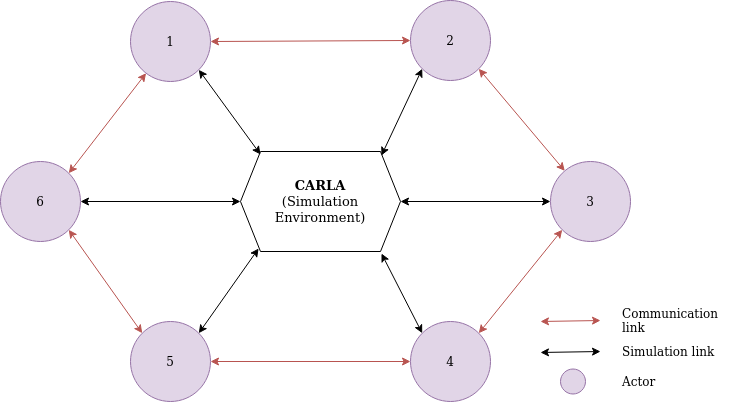
\includegraphics[width=8cm]{Framework/Images/Arc1.png}.
    \caption{Simulation Environment}
    \label{fig:my_label}
\end{figure}

\section{Motivation}
Transportation is essential for our economy and society. A country's economic, social, and political life depends upon an effective transport system. Transport is a cornerstone of European integration and crucial for the free flow of citizens, services, and goods to be served. It is also a significant contributor to the economy, accounting for about 664 billion Euros in Gross Value Added in 2017 (i.e. 5\% of the total EU's GVA) and employed over 11 million people \cite{001}. 

According to the “Statistical pocketbook 2019” of European Commission \cite{001}, 50.1\% of total freight transportation were made via roadways. Nearly 73\% of passengers made their journey through road and among them, almost 90\% of them made the road trip by car. These statistics help us to understand the importance of roadways. The increase in traffic volume creates demand and eventually leads to traffic congestion across the EU. Due to traffic congestion, a driver spends approximately 28 hours in traffic every year. Additionally, it also creates environmental and economical impacts.

Traffic congestion usually occurs when traffic flow exceeds the road capacity. Many factors can cause traffic congestion, but infrastructure stands at the top.  A simple traditional solution to reduce congestion is expanding the infrastructure. However, this is not an effective or economically reasonable solution because one cannot keep on extending as demand increases. Preferably, utilizing the infrastructure capacity to the fullest is more efficient and rational. 

ITS helps us to address congestion by continuously monitoring and regulating the traffic flow. For instance, consider a junction with traffic signals that have fixed time to switch signal. They are only effective for the ideal traffic flow, when the traffic flow decreases
the driver has to wait till green and the traffic signal creates congestion as the traffic flow increases. On the other hand, ITS can help the traffic signals dynamically adjust the switching time depending on the traffic flow.

ITS components are installed in the vehicles and along the roadside to collect traffic data, guide and control the flow. Real-world traffic scenarios are complex, highly dynamic. Because of these reasons, it must be tested and evaluated before real-world deployment. Else, they may lead to a serious problem instead of avoiding congestion. 

Including a simulator in the development cycle of ITS will help us to evaluate the system in all possible scenarios by testing it in the simulation environment mirroring real-world ITS.  Using simulators to test and evaluate ITS is cost-effective and risk-free compared to build a real-world test site.

\section{Project Overview}
\subsection{Intelligent Transportation System}
A set of different applications that use state-of-the-art technologies to monitor and regulate the traffic flow are known as ITS. Throughout the world, many countries have designed and developed ITS, and they have unique visions and goals to improve infrastructure applying ITS. Despite counties having different perspective toward ITS, they share the common goal to improve the current transportation infrastructure. This dissertation follows the standards and architecture of ITS proposed by the European Union \cite{etsi}.

\subsection{Approach}
To simulate the ITS, we need a road network, traffic infrastructure, mobility model to control vehicle behaviour, traffic demand to generate traffic flow and network model to create a communication infrastructure. 

Traffic simulators like SUMO \cite{SUMO2018}, PVT-Vissim \cite{vissim}, etc.  can create road infrastructure and simulate traffic flow based on demand and vehicle behaviour, but they do not support communication between vehicles. On the other hand, network simulators like ns3 \cite{ns3}, OMNET++ \cite{omnet}, etc. can create network infrastructure and simulated realistic communication, but they do not support mobility. Therefore, traffic simulators and network simulator should be coupled through a TCP link to create an ITS simulation environment. 

The above-mentioned simulators have to be extended for developing a customised TMS like Cooperative Adaptive Cruise Control (CACC) \cite{cacc}, platooning, slot-based driving \cite{slot-based}, etc.  For example, PLEXE \cite{plexe} implemented a platooning application by extending the Viens\cite{veins} framework (Viens is a vehicular network simulation framework created by coupling SUMO and OMNET++). The framework to simulate the ITS environment for developing TMS will be similar to the figure. 

This framework performs space-continuous and time-discrete simulation ( i.e. it updates the simulation after every time step). 
After each time step, the traffic simulator computes the behaviour of all vehicles based on the network simulation results to update the vehicle states and generate movement trace. Then, it sends the movement trace to network simulator. The network simulator updates the position of all nodes based on the received movement trace, simulates the communication and sends the result back to the traffic simulator. The sequence diagram in the figure illustrates this process. The approach lacks implementing the distributive nature of ITS and can only perform time-discrete simulation, but in real scenario time is continuous.

This dissertation introduces a framework that uses only Carla, autonomous driving simulator for simulating ITS. The framework is created by extending the Client API of Carla. Based on the traffic demand, vehicles are added as Carla client using the framework. The distributed network formed by the clients creates the communication infrastructure. 

In the proposed approach, peer to peer socket communication is used to exchange messages instead of simulating it. Each client node is responsible for its behaviour computation based on the messages it receives. This framework is capable of performing a time-continuous simulation with the help of Carla Server's asynchronous mode. Thus, it can be used to create a more realistic ITS simulation.


\subsection{Research Aims}
The research intends to design and develop a simulation framework for ITS, that creates a realistic and distributed simulation environment. The main motive is to help developers to concentrate on developing and evaluating traffic management system (TMS) models. Apart from the above, the specific objectives of this dissertation is to evaluate the feasibility of the proposed approach by creating customised scenarios using the designed framework

\subsection{Project Scope}
The dissertation focuses on designing a approach to developing a simulation framework using only an autonomous driving simulator
to create an environment closely resembling real-world ITS. Especially focuses on simulating and evaluating an actor's behaviour while developing new traffic management systems in a distributed environment. 

The framework distributes computation of the actor's behaviour among several nodes in a network and exchanges information between them through socket communication. This dissertation is not concerned about implementing the network infrastructure or underlying protocols involved in vehicular communication. 
\subsection{Benefits of this Research}
The benefit of this research is to improve the testing and evaluation processes involved while developing TMS and ITS. 
\subsection{Road Map}
The rest of this dissertation is divided into four parts, starting with chapter 2 that provides the necessary background information for this work and the state-of-the-art simulation framework for testing ITS. Chapter 3 is about the design of the framework and decisions that lead to the development of the proposed approach. The following chapter explains the architecture of the framework and APIs provided for creating custom scenarios using the framework. Chapter 5 will discuss the evaluation of the framework. Finally, the dissertation concludes with an outline stating the pros and cons of this work and future work to enhance the framework.

  \chapter{Background}
    This chapter discusses the required background information needed for a better understanding of the proposed work. In the first section explains the overall architecture of ITS and their components. The second section discusses the current state-of-the-art techniques used to perform ITS simulation. At last, an overview of the tools used to build the framework is given.
\section{Intelligent Transportation System}
\begin{figure}[h!]
    \centering
    
    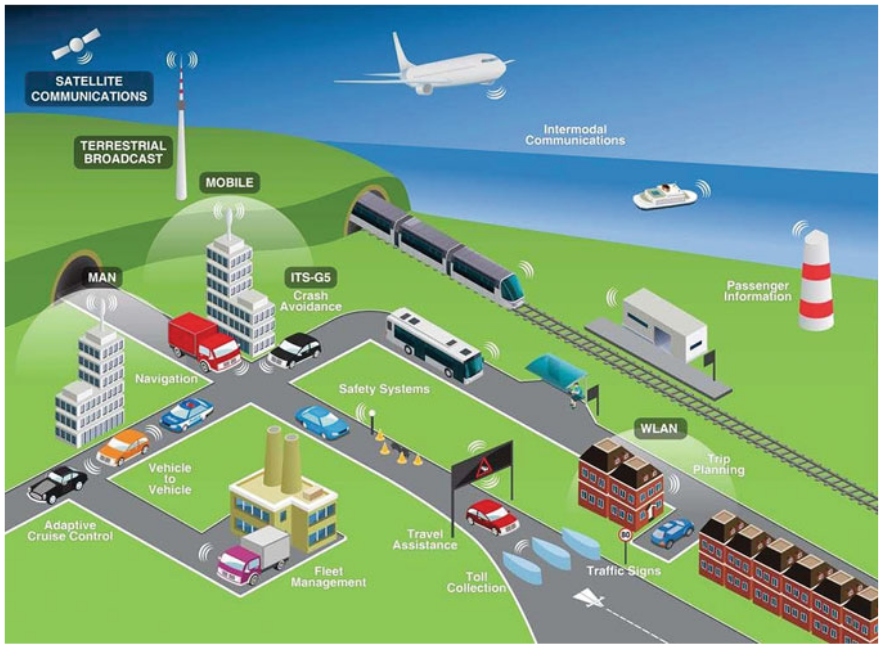
\includegraphics[width=10cm]{Framework/Images/CITS.png}.
    \caption{C-ITS Environment \cite{etsiDENM}}
    \label{cits}
\end{figure}

The Intelligent Transportation Systems (ITS) comprises of different applications that improve the safety, security and efficiency of transportation and provide a better driving experience. ITS achieves this by gathering necessary data from the sensors or devices placed in the infrastructure or vehicles. Initially, ITS only provided intelligence to vehicles  and roadside infrastructure, it was not able to share information between them and make them cooperate to regulate the traffic. 
The European Commission introduced the Cooperative Intelligent Transportation System as a new category of ITS \cite{alam_ferreira_fonseca_2016}. In which drivers, vehicles, passengers or road operators can directly interact with each other or with the surrounding infrastructure and figure \ref{cits} illustrates a typical CITS environment. CITS takes advantage of the communication and cooperation between different actors and effectively regulate the traffic flow by exchanging information about traffic jams, congestion, accidents. 

\subsection{Architecture}
Intelligent Transportation System consists of four sub-systems or stations \cite{etsi}, that helps transportation infrastructure to gain intelligence and real-world information . All the Sub-Systems are made up of ITS Station (ITS-S), it may contain a single ITS-S or network of ITS-S. 

\subsubsection{ITS Station Reference Architecture}
The ITS Station is the base component upon which a sub-system is built and its reference architecture helps to understand the functionality of ITS Station. Its architecture follows the principles of the OSI model\cite{OSI} for the layered communication protocol, and it is extended to include different ITS applications. In the figure \ref{ci88ts-s},

\begin{itemize}
\item Access layer is responsible for the functionality of Physical and Data Link layers
\item Network and Transport layer is responsible for the functionality of  Network and Transport layers
\item Facilities layer is responsible for the functionality of Session, Presentation and Application layers
\item Application layer
\item Management layer is responsible for managing the communication with the ITS Station
\item Security layer is responsible for providing security services to ITS Station and it is also considered as a part of  management entity.
\end{itemize}

\begin{figure}[h!]
    \centering
    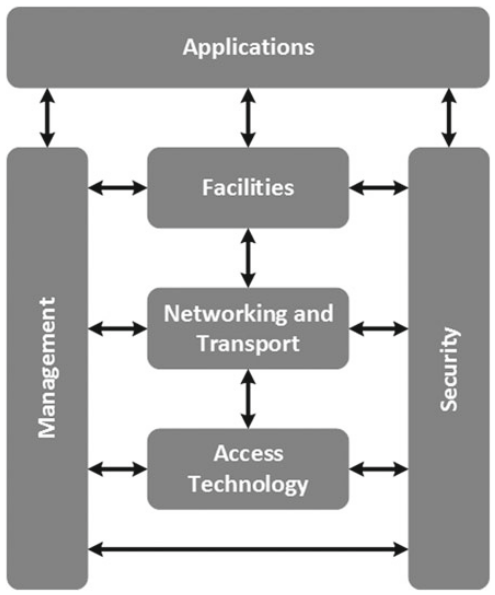
\includegraphics[scale=0.40]{Framework/Images/ITS-SRefArc.png}.
    \caption{ITS Station Reference Architecture }
    \label{ci88ts-s}
\end{figure}

\subsubsection{Functional Components of ITS Station}
 Based on their functionality, ITS Station can be divided into four sub-clauses \cite{etsi}
\begin{itemize}
    \item \textbf{Host :} It helps to run the ITS application
    \item \textbf{Gateway :} It helps to connect a ITS Station with the external propriety network. Facilities layer helps to connect different protocols.
    \item \textbf{Router :} It helps to connect one ITS Station with another. Network and transport layer helps to connect different ITS-S.
    \item \textbf{Border Router :}  It is similar to router but it can also connect ITS-S with external network.
    
\end{itemize}

\subsubsection{ITS Sub-Systems}

\begin{itemize}
    \item \textbf{Personal Sub-Systems/Station} help us to access ITS applications or platform through smartphones, Human Machine Interface or similar devices. They can be used as a user interface for crowdsourcing, getting feedbacks or as an interface for other sub-systems or station. Its internal network contains only ITS-S host.
    \item \textbf{Roadside Sub-Systems/Station} are placed along the roadside to collect real-time traffic (e.g. traffic flow, volume, etc.) and environment (e.g. temperature, wind speed, humidity, etc.) information, acts as a gateway or a router for other ITS Sub-Systems and controls equipments like a traffic signal, electronic signboards, etc to provide assistance to the drivers. Its internal network contains ITS-S host, gateway, router and border router. 
    \item \textbf{Vehicle Sub-Systems or Station} are installed in the vehicles and connected to their proprietary vehicular network (e.g. CAN bus). They accumulate information about the vehicle, their surrounding and drivers trip details. It can be used to control the vehicle during an emergency situation. They provide the collected information to the driver and other Sub-Systems. Its internal network contains ITS-S host, gateway and router.
    \item \textbf{Central Sub-Systems or Station} are used to monitor the other Sub-System.
    
\end{itemize}

\begin{figure}[h!]
    \centering
    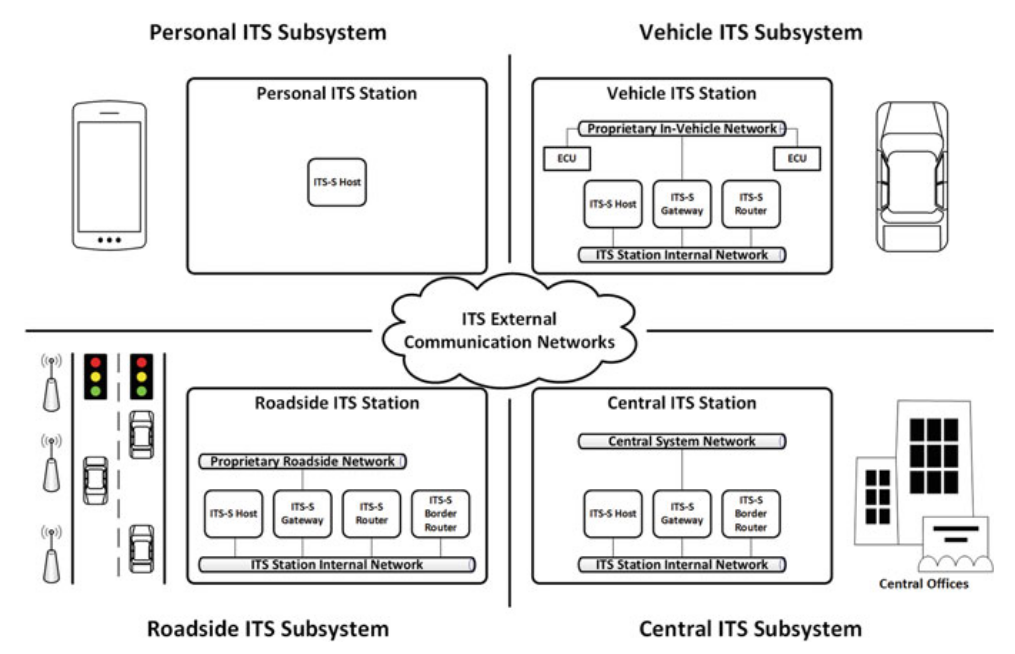
\includegraphics[width=12cm]{Framework/Images/ITSArc.png}.
    \caption{European ITS communication sub-systems}
    \label{cits---s}
\end{figure}
\subsection{Vehicular Communication}
As mentioned above, vehicular communication plays a vital role in ITS to establish cooperativeness and sharing information.  It is implemented using communication technology based on WAVE/IEEE 802.11p \cite{WAVE}. Depending on the Subsystem a vehicle communicates with the modes are divided into three:

\begin{itemize}
    \item \textbf{Vehicle-to-Vehicle (V2V): } In this mode it communicates with another vehicle.
    \item \textbf{Vehicle-to-Roadside Infrastructure (V2R): } In this mode it communicates with the roadside infrastructure.
    \item \textbf{Vehicle-to-Everything (V2X): } In this mode it can communicate with device in the traffic infrastructure.
\end{itemize}

\begin{figure}[h!]
    \centering
    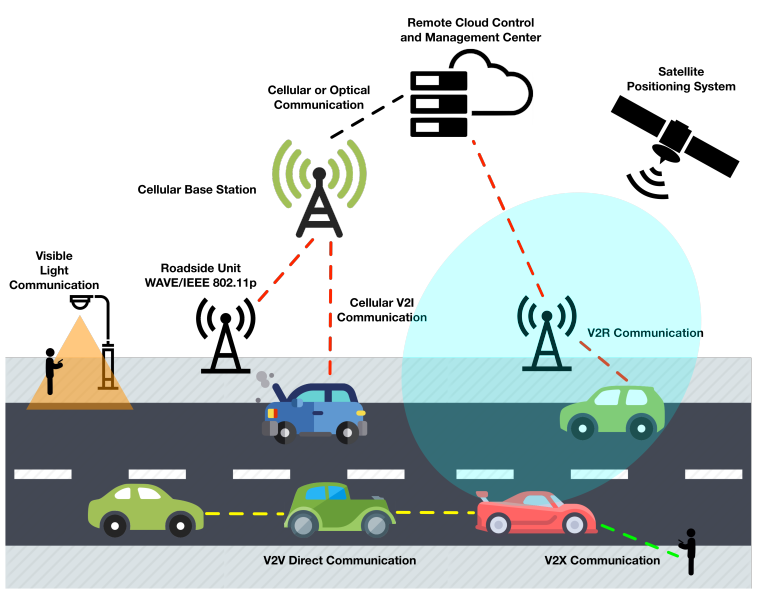
\includegraphics[width=12cm]{Framework/Images/communicationModes.png}.
    \caption{Vehicular Communication Modes \cite{vComs}}
    \label{comsMode}
\end{figure}
\subsection{Cooperative Awareness Message (CAM)}
Cooperative Awareness Message (CAM) \cite{etsiCAM} is a part of the basic cooperative services that are available in all  ITS Stations. CAM is similar to a beacon that is exchanged between an ITS-S and its neighbours to make them aware of their surrounding environment and to enable cooperativness between them. CAM is generated and transmitted periodically but the frequecy is determined by the generating station. 

The content provided by a CAM may vary depending on ITS-S type by all the messages contains the reference position, status and type of the station generating the message. CAM is only transmitted to the stations that are within the communication range of the orginating station and they are not forwarded to other stations once received.
\subsection{Decentralized Environmental Notification Message \\(DENM)}
Decentralized Environmental Notification Message (DENM) \cite{etsiDENM} is a part of basic cooperative service to support the Road Hazard Warning (RHW) application and available in all the ITS stations. DENM is used to notify and warn ITS Stations and users about events that are hazardous to the traffic flow (i.e. vehicle breakdown, accident, lane status, etc..). ITS application triggers and generates DENM upon the occurrence of an event. DENM transmission is repeated and lasts until the triggered event is resolved. A DENM broadcast is terminated once the predefined time limit set by CA service expires or by the ITS application that triggered the DENM.

The DENM contains information about the event that triggered it along with the type and location of the event. DENM are broadcasted through vehicle-to-vehicle (V2V) and vehicle-to-infrastructure communication. Once received, a station forwards the DENM to other stations and only shows the relevant notifications to the driver.

\section{ Current State of the Art in ITS Simulation}
Veins is a popular vehicular network simulation framework researchers use for ITS simulation and evaluation. In this paper \cite{ITSref}, they created an C-ITS applications by extending it to evaluate the application's Quality of Service (QoS). An overview of Viens and its simulation technique is briefly described in the next section before discussing the paper.

\subsection{Veins}
Viens is a simulation framework that performs vehicular communication simulation. It uses OMNET++, discrete-event network simulator and SUMO, discrete-time traffic simulator and binds them using Traffic Control Interface (TraCI) a protocol based on TCP socket. Veins simulate both OMNET++ and SUMO parallelly, and TraCI creates a bidirectional-coupling and make the simulators interact with each other. 

SUMO simulate traffic based on the demand and generates movement trace and sends it to OMNET++. Then, the network simulator updates all the nodes based on the movement trace simulates communication and sends back the simulation result to SUMO.

Viens implemented vehicle and roadside ITS subsystem as network entities to perform vehicular communication. Each entity contains three components and they are extended to create new ITS application, the components are
\begin{itemize}
    \item \textbf{Network Interface Card (NIC): } It implements protocols and stack required vehicular communication
    \item \textbf{Mobility: } It is responsible for the mobility of the network entity, it configures the position based on the movement trace for a vehicle or a static position for RSU 
    \item \textbf{Application: } It implements application, that generates and shares message based traffic information  to perform a basic simulation.
\end{itemize}

\subsubsection{Bidirectionally Coupled Simulation}
Viens extended both the simulators and added a communication model to exchange and buffer commands and messages ( e.g., simulation results, movement trace).  

Since OMNET++ is a discrete-event simulator, it should be triggered to perform the simulation. The framework schedules a trigger at a regular interval to update the node movement and perform the simulation. It follows the same trigger approach for SUMO, as it is a discrete-time simulator the approach suits well. The communication module buffers any messages received by the simulators until the next trigger. 


\begin{figure}[H]
    \centering
    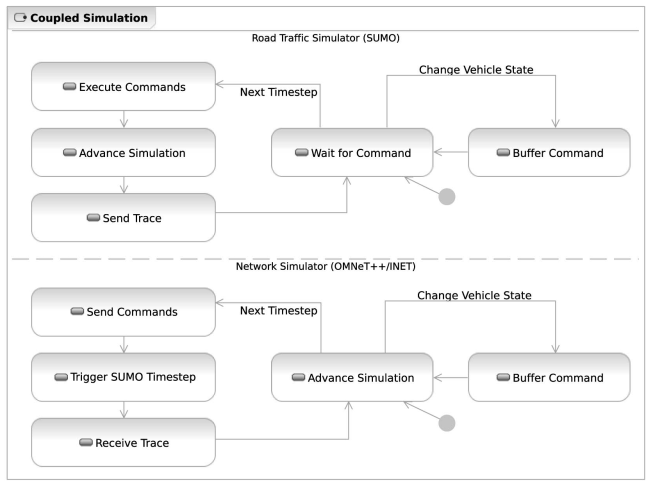
\includegraphics[width=12cm]{Framework/Images/veins1.png}.
    \caption{ Flow Diagram of the simulation \cite{veins}}
    \label{v1}
\end{figure}

\begin{figure}[H]
    \centering
    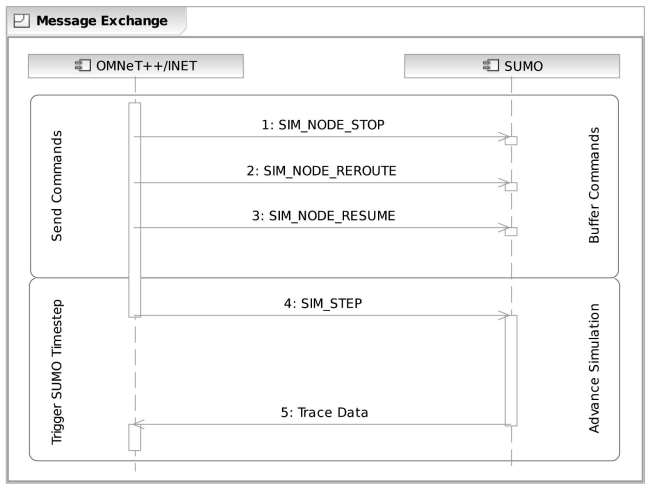
\includegraphics[width=12cm]{Framework/Images/veins2.png}.
    \caption{ Sequence diagram of messages exchanged between simulators \cite{veins}}
    \label{v2}
\end{figure}

At each time step, OMNET++ sends the simulation result as commands and trigger to SUMO, then SUMO performs traffic simulation. After the simulation, SUMO sends the generated movement trace back to OMNET++ and waits for the next trigger. This way OMNET++ updates the position of all the nodes based on the movement trace received from SUMO and performs simulation until the next trigger. During the simulation, OMNET++ makes its nodes interact with inter-vehicle communication and reassign their attributes (e.g., speed, route). In this process, SUMO computes the behaviour of each vehicle in the traffic based on the attributes (e.g., speed, route) of the corresponding nodes. Figures \ref{v1} and \ref{v2} illustrates the entire process.


\subsection{Extending Veins for ITS Application Simulation}
Veins is extended to implement multiple ITS application to evaluate the  QoS of the message broadcasting model. The applications implemented are:
\begin{itemize}
    \item Hazard warning (HW), an event-driven road Safety application
    \item Dynamic speed limit (DSL), a traffic management application
\end{itemize}

First, they create the Traffic Manager Control (TMC) application entity class, it is inherited from BaseWAVEApplLayer class. Then they override the custom application component of Veins RSU with TMC. Now, Veins RSU is customised to send HW and DSL messages. Likewise, the application component of the vehicle entity is overridden with CarApps class. Now, Venis is fully extended and ready for the ITS simulation

\begin{figure}[h!]
    \centering
    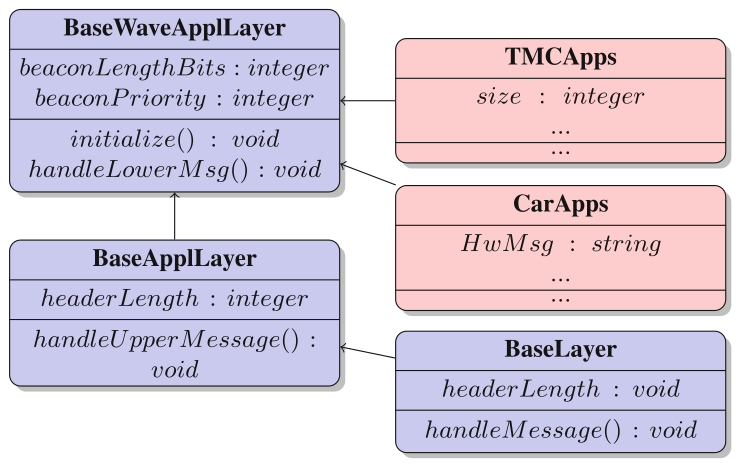
\includegraphics[width=8cm]{Framework/Images/veinsExt.png}.
    \caption{ class of TMC and CarApps  \cite{veins}}
    \label{vExt}
\end{figure}

\section{Tools}
This section discusses the various tools used by the framework to perform the simulation. The framework uses Carla Server as a simulation engine and CarlaViz to visualize the entire simulation in a webpage.
\subsection{CARLA}
\say{CARLA is an open-source autonomous driving simulator} \cite{carla_simulator_2020}. It provides a set of API to perform autonomous driving simulation and build as a tool to help researchers and companies to \say{democratize autonomous driving R&D} \cite{carla_simulator_2020}. It used the Unreal Engine to compute physics and perform simulation and follows the OpenDRIVE standard to design road network and related settings. The simulation performed by the Unreal Engine is controlled by its API provided by Carla in Python and C++. Apart from autonomous driving R&D,  this is a great tool to simulate mobility.

\subsubsection{Architecture}
Carla is built based on a client-server architecture pattern. The server is coupled with the Unreal Engine, and it holds sole responsibility for simulation (i.e., physic computation, sensor and scene rendering are performed). The server is divided into two components based on the elements they control in the simulation. The figure \ref{carc} illustrates the architecture of Carla. 

\begin{itemize}
    \item \textbf{World Server: } This component is responsible for creating the simulation environment. This includes the building, road network, actors (vehicles, sensors and other static properties) etc. It is used to initiates sessions to perform the simulation. Once, initiated it sets the simulation world where actors can be placed.
    \item \textbf{Agent Server: } This component is responsible for the simulating actors. It provides two threads, Control Thread (It receives commands for simulation from a client) and   Measurements Thread (It streams the live sensor data from the simulation).
\end{itemize}

The Carla Server only creates the platform and provides the infrastructure for performing the simulation. The behaviour of all the element is controlled by the Carla Client. A user can gain complete control over an actor, starting from creating it and controlling their behaviour throughout their lifetime. 

\begin{figure}[h!]
    \centering
    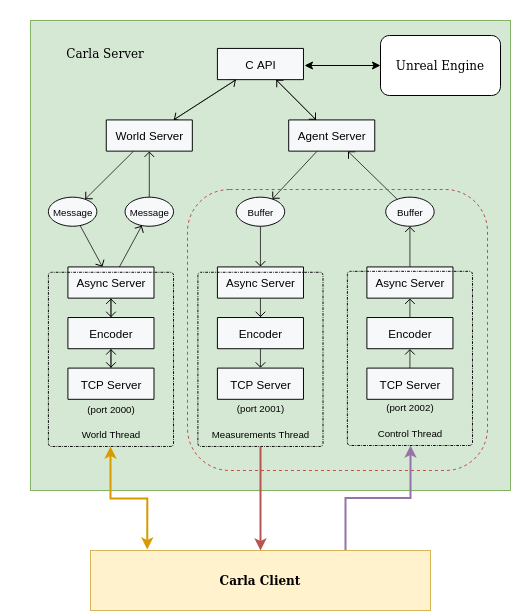
\includegraphics[width=12cm]{Framework/Images/carlaArc.png}.
    \caption{Carla Architecture \cite{carla_simulator_2020}}
    \label{carc}
\end{figure}

\subsubsection{Client-server synchrony}
This section explains about different modes of communication between a client and the server. The server runs in Asynchronous mode by default. In this mode, it simulates as fast as possible without does not wait for any client. On the other hand, in Synchronous mode, the server waits for the client. It proceeds to simulate only if the client gives the signal to do it.

The client can also control the simulation time-step. By default, the server does not follow a fixed time gap, it is called "Variable time-step". The time gap depends on the computation and rendering of physic. The simulation time-step can be fixed by a client. Based on this the server can perform a time-continuous and time-discrete simulation. The figure \ref{carm} shows all the configuration modes provided by Carla.

\begin{figure}[h!]
    \centering
    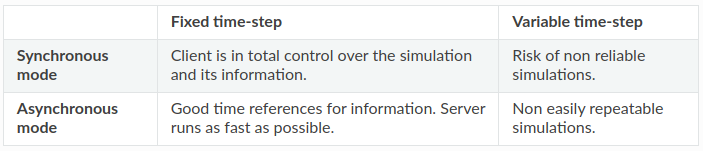
\includegraphics[width=12cm]{Framework/Images/carlaModes.png}.
    \caption{Configuration Modes Provided by Carla \cite{carla_simulator_2020}}
    \label{carm}
\end{figure}

\subsection{CARLAVIZ}
Carlaviz is a visualization plugin developed for Carla to view the simulation environment through a web browser. It streams the world created by the server along with the actors (i.e. Vehicles and pedestrians) living in them and updates their status on the air. Along with this, it streams data from the sensors and visualizes using tables and graphs. Added to this, Carlaviz also allows users to draw texts, points and lines on the visualization. The figure is the sample screenshot of the visualization.

\begin{figure}[h!]
    \centering
    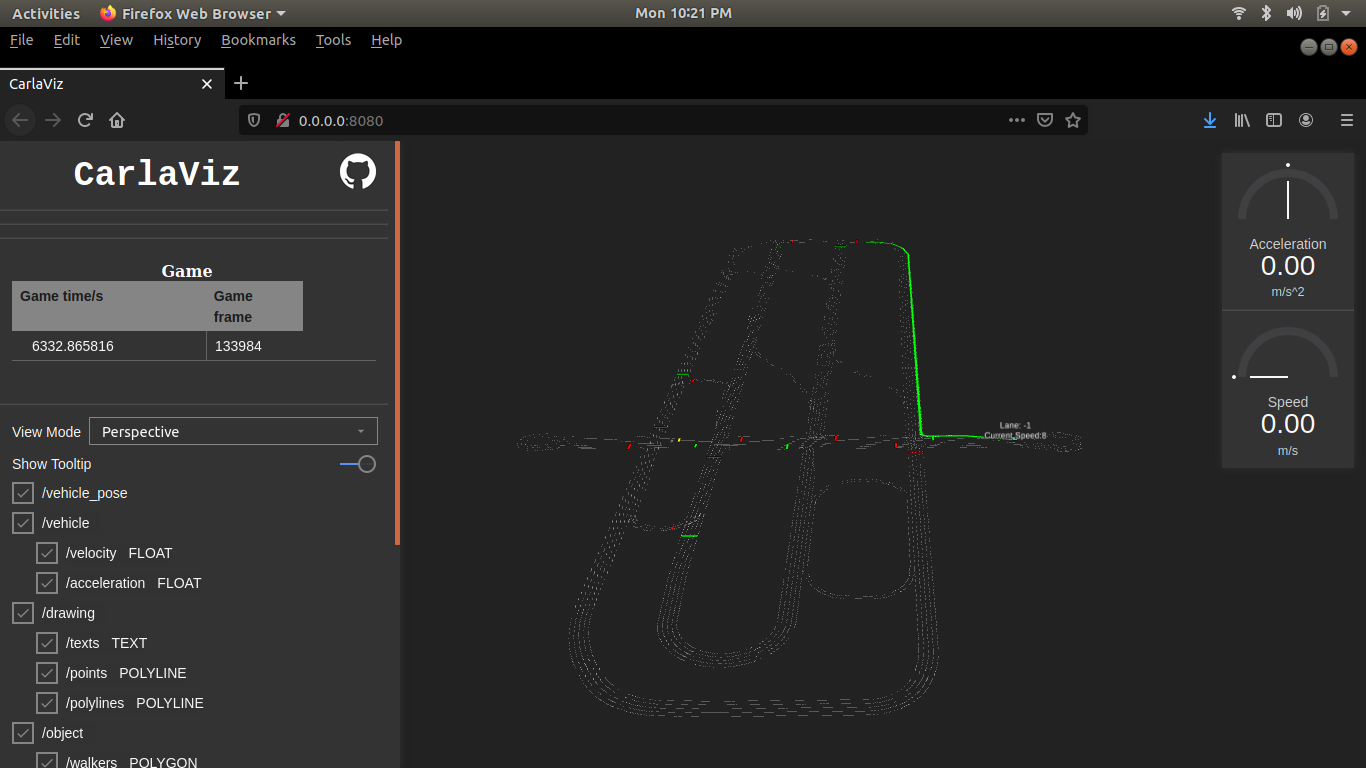
\includegraphics[width=15cm]{Framework/Images/caraVIZ.png}.
    \caption{CarlaVIZ Visualisation Screenshot}
    \label{carm}
\end{figure}

  \include{chapter3}
  \include{chapter4}
  \include{chapter5}
  \include{chapter6}
  

%\begin{thebibliography}{refs}                   %% Start your bibliography here; you can
\bibliographystyle{ieeetr}
\bibliography{refs}                               %% also use the \bibliography command
%\end{thebibliography}                             %% to generate your bibliography.


\addcontentsline {toc}{chapter}{Appendices}       %% Force Appendices to appear in contents
\begin{appendix}
 \chapter*{Appendix 1}

This appendix contains the class diagram of the framework. It is divided into three parts:
\begin{figure}[h!]
    \centering
    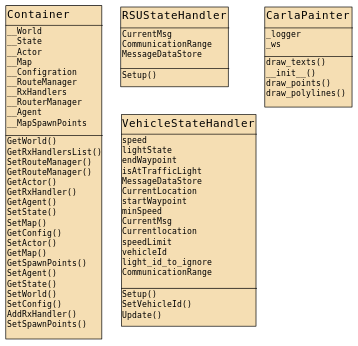
\includegraphics[width=10cm]{Framework/Images/CD2.png}.
    \caption{Class Diagram of Helper Component}
\end{figure}
\begin{figure}[h!]
    \centering
    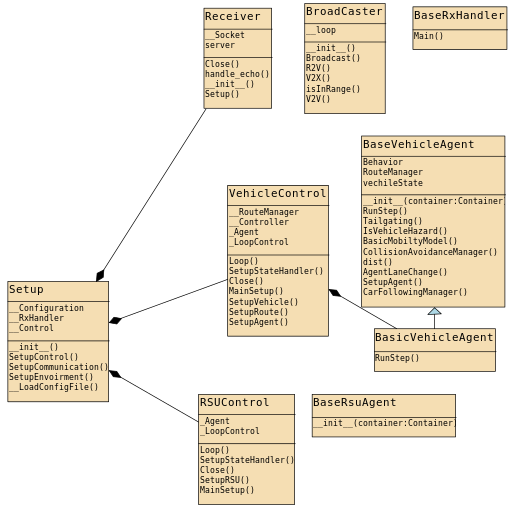
\includegraphics[width=15cm]{Framework/Images/CD1.png}.
    \caption{Class Diagram of Setup, Control and Communication Components}

\end{figure}

\begin{figure}[h!]
    \centering
    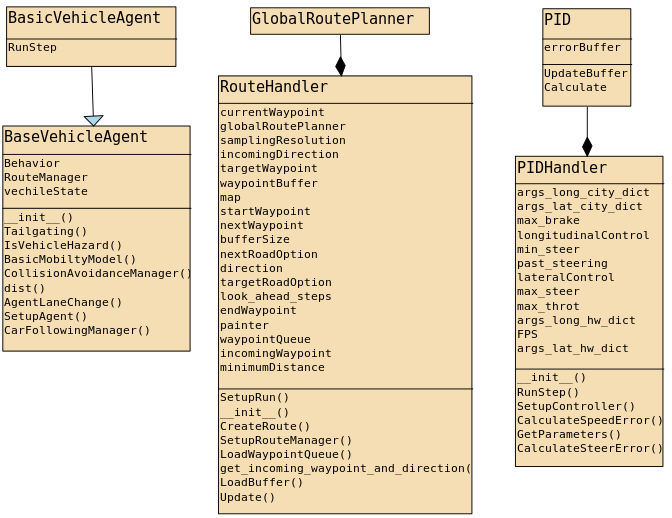
\includegraphics[width=15cm]{Framework/Images/CD3.png}.
    \caption{Class Diagram of Vehicle Control Class}
\end{figure}


 \chapter*{Appendix 2}
This appendix contains code snippets of the two scenarios implemented by extending the designed framework

\begin{figure}[h!]
    \centering
    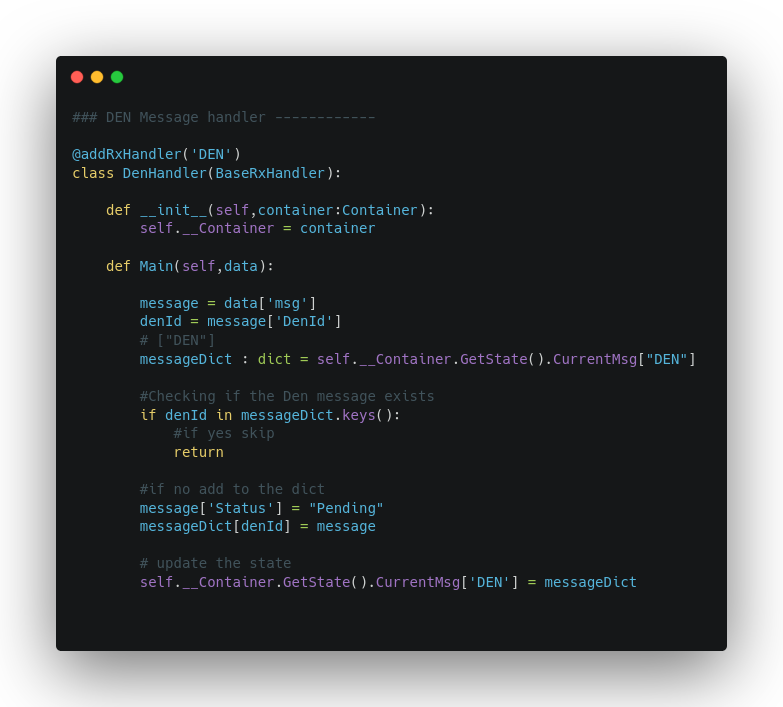
\includegraphics[width=12cm]{Framework/Images/denMH.png}.
    \caption{Code Snippet of DEN Message Handler}
\end{figure}

\begin{figure}[h!]
    \centering
    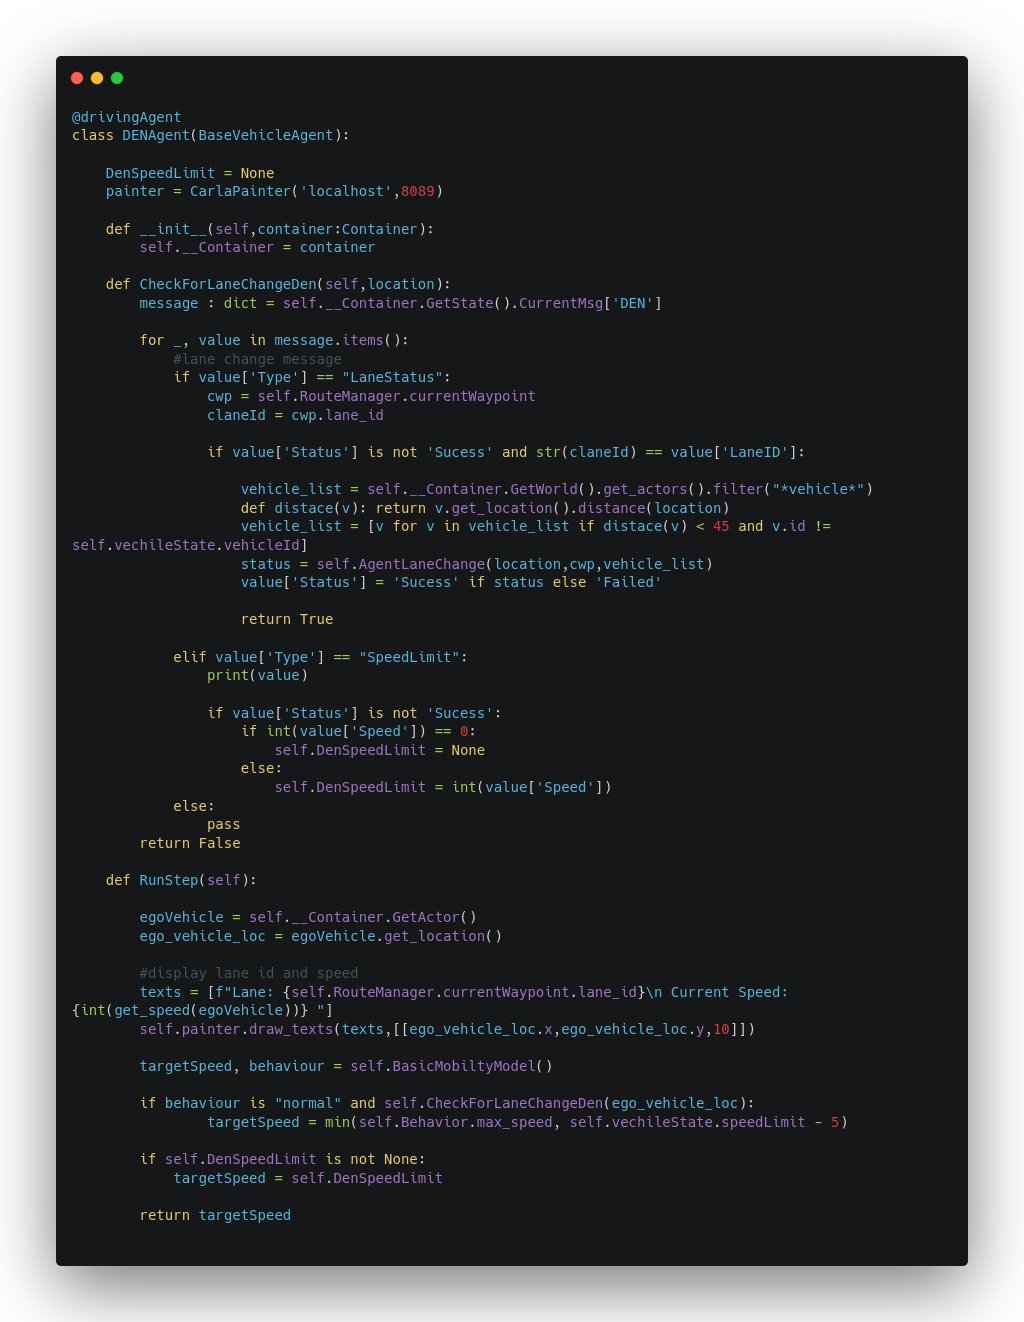
\includegraphics[width=15cm]{Framework/Images/denV.png}.
    \caption{Code Snippet of DEN Vehicle Behaviour}
\end{figure}
\begin{figure}[h!]
    \centering
    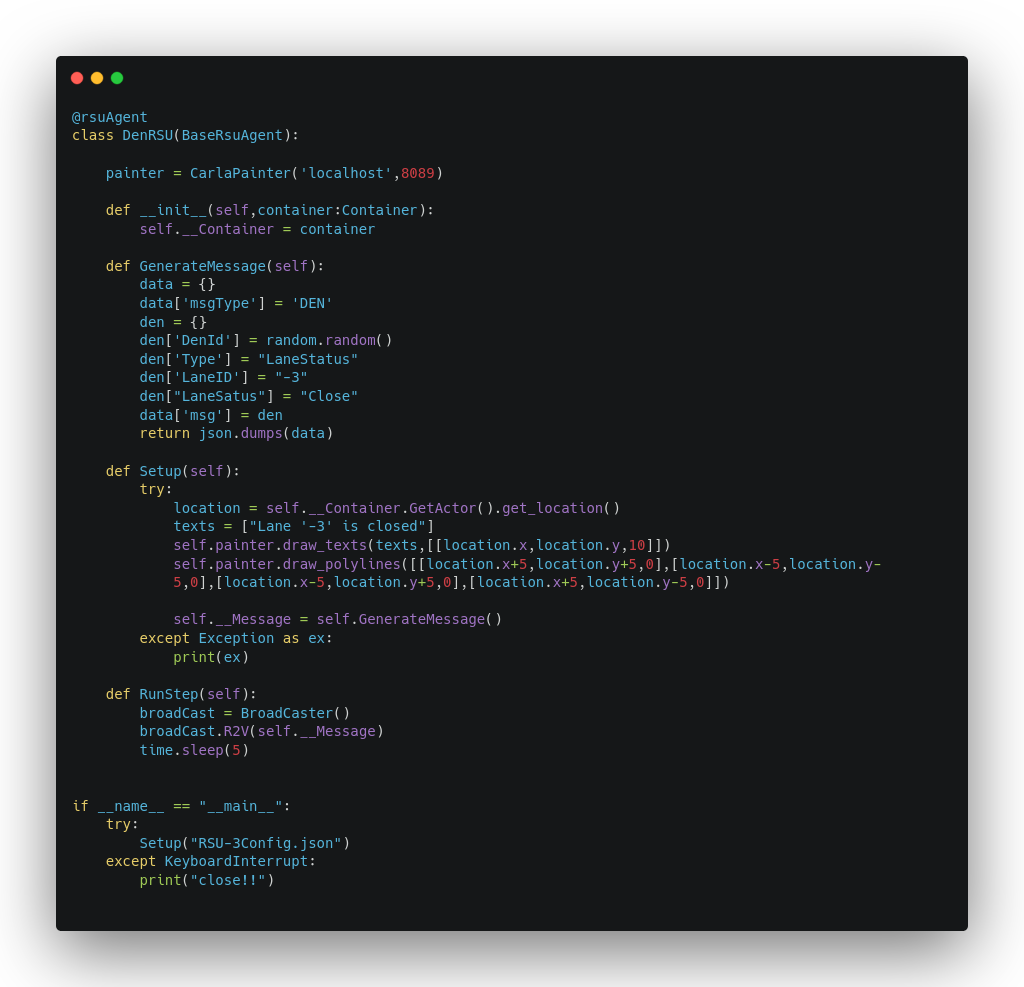
\includegraphics[width=15cm]{Framework/Images/denRSU.png}.
    \caption{Code Snippet of DEN RSU Behaviour}
\end{figure}

 \chapter*{Appendix 3}
This appendix contains screen shot of the DENM exchange scenario. In this simulation the vehicle initially moves in lane \say{-7} and when it comes in the communication range of RSU, it receives the lane closes message and it initiates lane change and moves to lane \say{-6} and at last when it comes near last RSU, it receives speed limit warning and reduces the speed

\begin{figure}[h!]
    \centering
    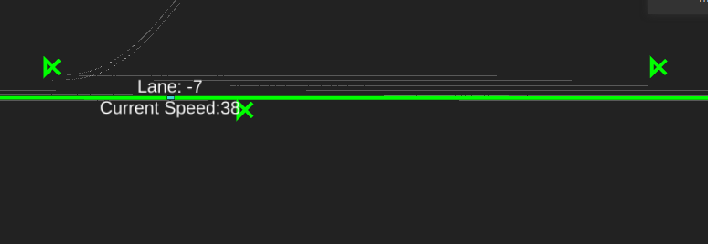
\includegraphics[width=12cm]{Framework/Images/1.png}.
    \caption{Scene 1: initially moves in lane '-7'}
\end{figure}
\begin{figure}[h!]
    \centering
    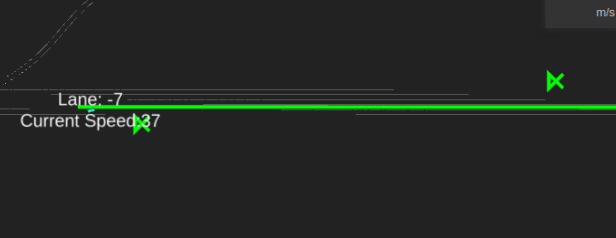
\includegraphics[width=12cm]{Framework/Images/2.png}.
    \caption{Scene 2: initiates lane change}
\end{figure}
\begin{figure}[h!]
    \centering
    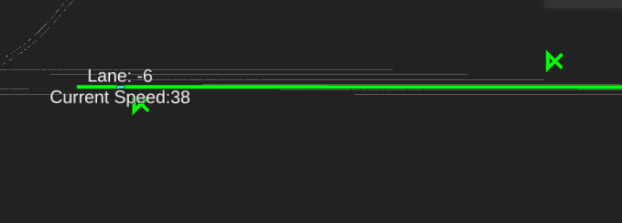
\includegraphics[width=12cm]{Framework/Images/3.png}.
    \caption{Scene 3: Changes the lane}
\end{figure}
\begin{figure}[h!]
    \centering
    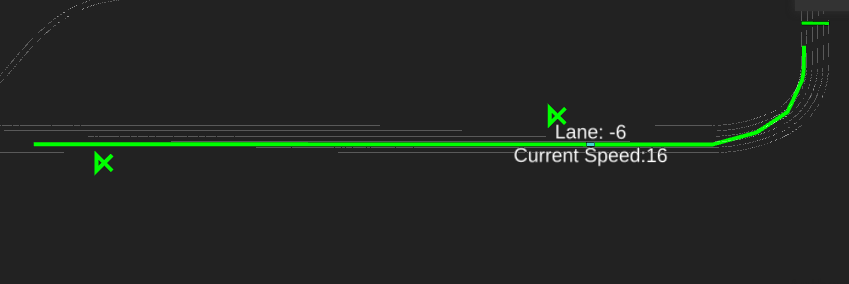
\includegraphics[width=12cm]{Framework/Images/4.png}.
    \caption{Scene 4: Reduces the speed}
\end{figure}
 \chapter*{Appendix 3}
\begin{itemize}
    \item \textbf{Project git repository :} https://github.com/amrishAK/ITS-Simulation-Framework
    \item \textbf{Installing Carla :} https://carla.readthedocs.io/en/latest/start\_quickstart/
    \item \textbf{Installing CarlaViz:} https://carla.readthedocs.io/en/latest/plugins\_carlaviz/
\end{itemize}
\end{appendix}


%\addcontentsline {toc}{chapter}{Bibliography}     %% Force Bibliography to appear in contents


\end{document}                                    %% END THE DOCUMENT
